\documentclass{article}
\usepackage{graphicx}
\usepackage{fancyvrb}

\begin{document}

In the previous section we have identified the type of goods present in our model. The identification and specification of financial products to be included in the model has the same importance and is performed in this section. 

This task is not trivial and we perform it by using  
%A characteristic of our model is the focus on the coherence at the stock level.
%This push us to use 
a stocks matrix approach that allows us to identify the type of financial assets needed to have a consistent framework. 

As we will explain later on in this section, using this approach we can also identify mechanisms to manage coherently situations of financial stress. The latter are important to study the functioning of the economy in pathological cases.  

To avoid inaccuracies in performing this thorny task, we start from a trivial representation where consumers and firms are present. We then gradually enrich the framework to obtain a configuration where government and banking sectors are also considered.

Before starting we recall that the stock matrix we will use hereafter reports the balance sheets of economic agents. 
Stock consistency implies that the sum of elements in each column and row of the matrix is zero.  


%Before progressing we present the simplest example. 
Let's consider an island-barter economy (money does not exist) populated by a single agent named Robinson Crusoe, whose main activity is to find food. 
The food in the island is perishable and inventories cannot be carried to the following periods. To perform his activity, Robinson establishes the Crusoe\&co to which he bestows his tools ($K$). From an accounting point of view we can distinguish two subjects: Robinson as a consumer and the Crusoe\&co. The balance sheets of the two subjects in the economy are represented as follows:

\vskip5mm
\begin{center}

\begin{tabular}{r c c}
	& \parbox{1.5cm}{\centerline{firm}} & \\
\hline
real	&$K$	& $+$	\\
(production capital)&		&	\\
\hline
financial&$EF$	&$-$	\\
\hline
&$\sum$		&0\\
\end{tabular}


\hskip1cm
\begin{tabular}{r c c }
	
	&household&\\
\hline
financial&$EF$	&	$+$  \\
\hline
counterbalance to financial &$WH$	&$-$\\
(wealth) &	&\\
\hline
&$\sum$	&	0
\end{tabular}


\end{center}
\vskip5mm
note that setting up an accounting framework creates two ``artificial'' categories: the counterpart to the production capital in Crusoe\&co balance sheet, $EF$, that we will call equity capital and the counterpart to equity capital in Robinson's balance sheet, $WH$, that measures his wealth. The signs are used to specify whether the component of the balance sheet is an asset $+$, or a liability $-$.

This reasoning allows us to identify a first category of financial assets: equity capital that %represents the value of $K$; 
in modern economies materializes in \textit{shares}.
With a change of perspective we say that both $K$ and $WH$ counterbalance the financial aspect so that the balance sheet of the two subjects can be summarized in the following stock matrix:

\vskip5mm
\begin{center}

\begin{tabular}{r c c}
	\hline
	& household 	& \parbox{1.5cm}{\centerline{firm}} \\
\hline
\hline
$EF$	&	$+$	&$-$	\\
	\hline
counterbalance to financial	&	$WH$	&$K$	\\
\hline
\hline
$\sum$		&0&0\\
\end{tabular}
\end{center}
\vskip5mm


It is worth emphasizing that the rows of the matrix relate to the types of assets that are accounted for in the economy.  In the simple case presented in this section, we consider only shares as financial assets.

\vskip5mm

As stated above, stock consistency implies that the rows of the matrix also sum to zero:

\vskip5mm
\begin{center}
\begin{tabular}{r c c c}
	\hline
	& household 	& \parbox{1.5cm}{\centerline{firm}}  &$\sum$\\
\hline
\hline
$EF$	&	$+$	&$-$	&0\\
	\hline
counterbalance to financial	&	$WH$	&$K$	&0\\
	\hline
	\hline
$\sum$ &	0	&0	&0
\end{tabular}

\end{center}
\vskip5mm

Let's consider a richer (and more populated) economy where someone invented a new contract. 
The Bank\&co is created to implement a business based on the newly created contract named bank account ($BA$). Both households and firms can sign a bank account contract with the Bank\&co.
 Households, firms and bank can be either lenders or borrowers. The lender records the $BA$ amount with a positive sign while the borrower with a negative sign. Note that the $BA$ amounts are usually referred to as either \textit{deposit}, if the household or the firm act as lenders, or \textit{loan} if they act as borrowers.  

Introducing this agent (the bank), two new financial activities are to be considered in the economy: its equity ($EB$) and the bank account. 
Concerning the latter, instead of using two different rows, one for deposits and one for loans, we think it is more coherent to use one line because the $BA$ is the unique contract an agent can sign with banks. This is of convenience because we will deal with a dynamic context in which a bank account changes its sign from period to period so that considering one entry rather than two will make the accounting easier.   

After considering the $BA$, the agents' balance sheets are:

\vskip5mm
\begin{center}

	\begin{tabular}{r c c }
	
		&\multicolumn{2}{c}{household}\\
\hline
&$BA$	&	$+/-$  \\
&$EB$	&	+  \\
&$EF$	&	+  \\
\hline
counterpart to fin. &$WH$	&$-$\\
\hline
&$\sum$	&	0
\end{tabular}
\hskip5mm
\begin{tabular}{r c c}
	& \multicolumn{2}{c}{firm} \\
\hline
&$BA$	&	$+/-$  \\
&$EB$	&	+  \\
&$EF$	&$-$	\\
\hline
counterpart to fin.	&$K$	& +	\\
\hline
&$\sum$		&0\\
\end{tabular}
\hskip5mm
\begin{tabular}{r c c}
	& \multicolumn{2}{c}{bank} \\
\hline
&$\sum BA$	&	$+$  \\
&$EB$	&	$-$  \\
&$EF$	&$+$	\\
\hline
counterpart to fin.	&	& 0	\\
\hline
&$\sum$		&0\\
\end{tabular}

\end{center}
\vskip5mm

Let us now build a stock matrix for an economy populated by one household, one firm and one bank. We consider the case in which $BA_h>0$, $BA_f<0$ and $BA_h>-BA_f$ and shares are held exclusively by households. The stock matrix is reported in table \ref{tab:sm1}.

\begin{table}
	\centering
\begin{tabular}{r c c c c}
	\hline
	& household 	& \parbox{1.5cm}{\centerline{firm}} & \parbox{1.5cm}{\centerline{bank}} &$\sum$\\
\hline
\hline
$BA$	&	$+$	&$-$	&$BA_h+BA_f$&0\\
$EB$	&	$+$	&	&$-$&0\\
$EF$	&	$+$	&$-$	&&0\\
	\hline
counterbalance to financial	&	$WH$	&$K$	&0\\
	\hline
	\hline
$\sum$ &	0	&0	&0
\end{tabular}
	\caption{stock matrix with $BA_h>0$, $BA_f<0$, $BA_h>-BA_f$ and shares are held exclusively by households}
	\label{tab:sm1}
\end{table}



A visual representation of the matrix is given in figure \ref{fig:vstock0}.
\begin{figure}[htp]
	\centering
\hskip-1cm
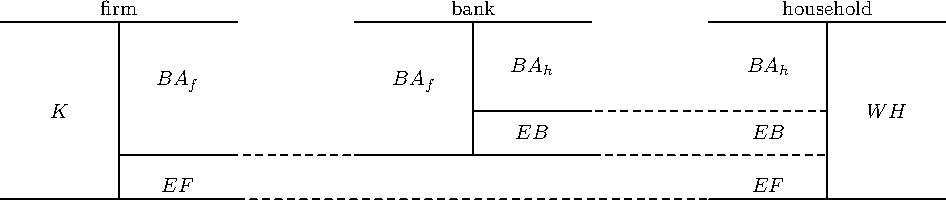
\includegraphics[scale=0.8]{balances-0.pdf}
	\caption{visual representation of the stock matrix}
	\label{fig:vstock0}
\end{figure}
It shows the result often highlighted in macroeconomic textbook that in this kind of economy, wealth equates production capital:
\[WH=K\]
but it also shows less straightforward relationships such as 
\[
	 K=BA_h+EB+EF
\]
or
\[
W=BA_f+EF
\]
A slightly more sophisticated case in obtained by letting banks and firm holding each other shares. The stock matrix is now reported in table \ref{tab:sm2} and visually represented in figure \ref{fig:vstock1}.

\begin{table}[t]
	\centering
\begin{tabular}{r c c c c}
	\hline
	& household 	& \parbox{1.5cm}{\centerline{firm}} & \parbox{1.5cm}{\centerline{bank}} &$\sum$\\
\hline
\hline
$BA$	&	$+$	&$-$	&$BA_h+BA_f$&0\\
$EB$	&	$+$	&$+$	&$-$&0\\
$EF$	&	$+$	&$-$	&$+$&0\\
	\hline
counterbalance to financial	&	$WH$	&$K$	&0\\
	\hline
	\hline
$\sum$ &	0	&0	&0
\end{tabular}
	\caption{stock matrix with $BA_h>0$, $BA_f<0$, $BA_h>-BA_f$ and shares are held by all the agents}
	\label{tab:sm2}
\end{table}

\begin{figure}[t]
	\centering
\hskip-1cm
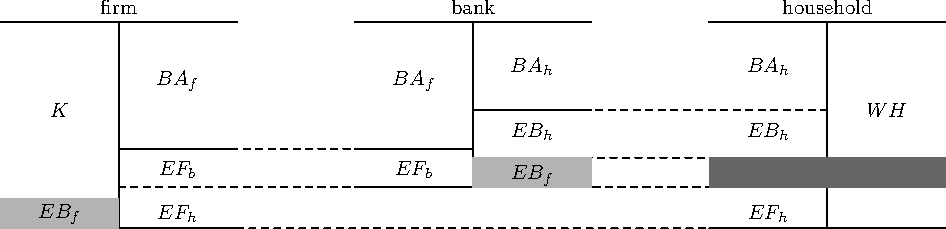
\includegraphics[scale=0.8]{balances-1.pdf}
	\caption{visual representation of the stock matrix}
	\label{fig:vstock1}
\end{figure}
The figure shows some gray area. They are introduced to find our relationships among balance sheet variables by visual inspection. In particular, the darker gray area signal areas that have to be discarded from the considered balance sheet while lighter ones are balance sheet items that are important for deducing relationships.  Consider for example firm assets. Their amount is given by
\[K+EB_{f}\]
looking now to household's liabilities we deduce that we have to add the dark gray area to wealth to reach the same amount of firm assets. But the dark gray area is equal to $EB_{f}$. So we can write
\[K+EB_{f}=WH+EB_{f}\]
that brings us to state that
\[WH=K\]
holds again. 
%In fact, to obtain the household's balance sheet we hat to remove the gray area. Its amount is equal to equity issued by the bank and hold by the firm ($E_{b,f}$). This is the same amount one have to subtract from the firm assets to obtain the production capital, thus $K=W$. 
As we did above, we can specify less straightforward relationships such as
\[K=BA_h+EB_{h}+EF_{h}\]
\[
	WH=BA_f+EF_{h}+(EF_{b}-EB_{f})
\]
that generalizes what written above.

We can now complete our framework by introducing the government. This also introduces an additional financial asset: government bonds ($GB$). 
Table \ref{tab:bsall} reports the balance sheets, table \ref{tab:sm3} the stock matrix and figure \ref{fig:vstock2} the visual representation of the new situation. 
We can again deduce the economic equations.
\[W+EB_{f}-GB_{f}=K+GB_b+GB_f+EB_{f}\]
\[WH=K+GB_b+GB_f+GB_{f}\]
\[WH=K+WG\]


\begin{table}[p]
	\begin{center}

	\begin{tabular}{r c c }
	
		&\multicolumn{2}{c}{household}\\
\hline
&$BA$	&	$+/-$  \\
&$EB$	&	+  \\
&$EF$	&	+  \\
&$GB$	&	+  \\
\hline
counterpart to fin. &$WH$	&$-$\\
\hline
&$\sum$	&	0
\end{tabular}
\hskip5mm
\begin{tabular}{r c c}
	& \multicolumn{2}{c}{firm} \\
\hline
&$BA$	&	$+/-$  \\
&$EB$	&	+  \\
&$GB$	&$+$	\\
&$EF$	&$-$	\\
\hline
counterpart to fin.	&$K$	& +	\\
\hline
&$\sum$		&0\\
\end{tabular}
\hskip5mm
\begin{tabular}{r c c}
	& \multicolumn{2}{c}{bank} \\
\hline
&$\sum BA$	&	$+$  \\
&$GB$	&	$+$  \\
&$EB$	&	$-$  \\
&$EF$	&$+$	\\
\hline
counterpart to fin.	&	& 0	\\
\hline
&$\sum$		&0\\
\end{tabular}
\hskip5mm
\begin{tabular}{r c c}
	& \multicolumn{2}{c}{government} \\
\hline
&$\sum GB$	&	$-$  \\
\hline
counterpart to fin.	&$WG$	& +	\\
\hline
&$\sum$		&0\\
\end{tabular}


\end{center}
	\caption{balance sheets with government bonds}
	\label{tab:bsall}
\end{table}



\begin{table}[p]
	\centering
\begin{tabular}{r c c c c c}
	\hline
	& household 	& \parbox{1.5cm}{\centerline{firm}} & \parbox{1.5cm}{\centerline{bank}} & \parbox{1.5cm}{\centerline{gov}} &$\sum$\\
\hline
\hline
$BA$	&	$+$	&$-$	&$BA_h+BA_f$&&0\\
$EB$	&	$+$	&$+$	&$-$&&0\\
$EF$	&	$+$	&$-$	&$+$&&0\\
$GB$	&	$+$	&$+$	&$+$&$-$&0\\
	\hline
counterpart	&	$WH$	&$K$&0&$WG$	&0\\
	\hline
	\hline
$\sum$ &	0	&0	&0&0
\end{tabular}
	\caption{stock matrix with $BA_h>0$, $BA_f<0$, $BA_h>-BA_f$ and shares are held by all the agents}
	\label{tab:sm3}
\end{table}

\begin{figure}[p]
\hskip-3cm
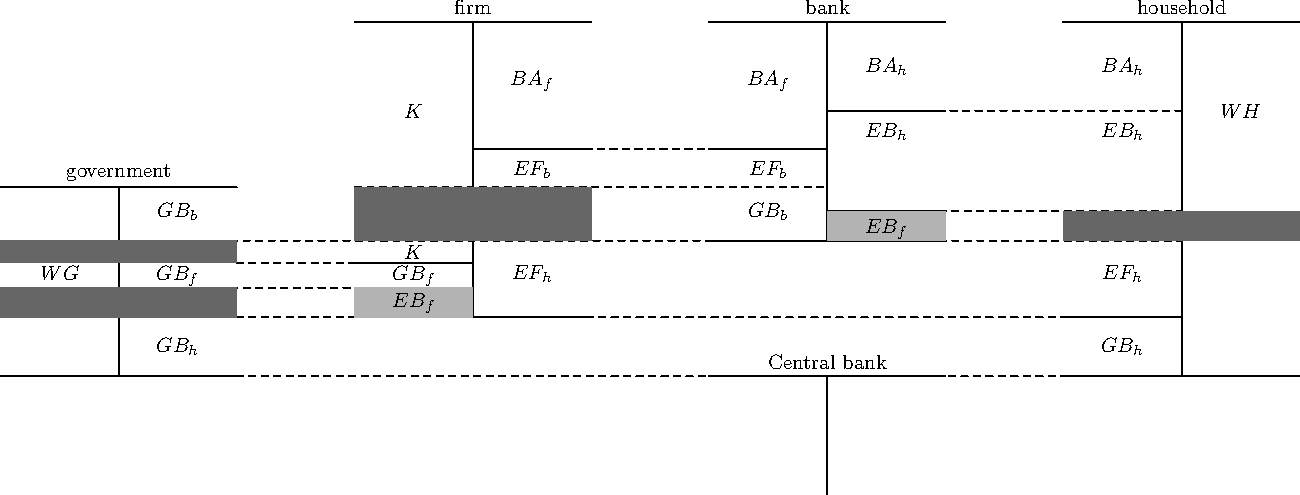
\includegraphics[scale=0.8]{balances-2.pdf}
	\caption{visual representation of the stock matrix}
	\label{fig:vstock2}
\end{figure}

\clearpage


Figure \ref{fig:vstock2} presents a rather complicate situation. We now simplify it to reach a starting point for considering situation of agents' financial stress. 
%We proceed by making two simplifications that brings us to our initial situation where shares are hold exclusively by households. 
The simplifications is: shares abd bonds are hold exclusively by households. 

Figure \ref{fig:vstock5} shows the simplified situation.   

\iffalse
\begin{itemize}
	\item the firm do not possesses bank shares
	\item the firm do not possesses government bonds
	\item the bank do not possesses the firm shares
\end{itemize}

represented in figures \ref{fig:vstock3} and \ref{fig:vstock4}.
Figure \ref{fig:vstock4} shows the simplified situation.   


\begin{figure}[p]
\hskip-3cm
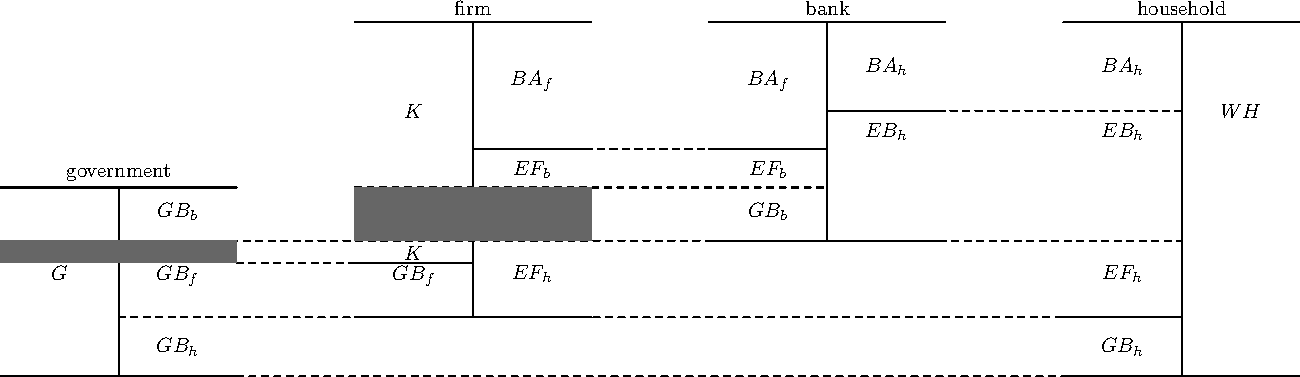
\includegraphics[scale=0.8]{balances-3.pdf}
	\caption{visual representation of the stock matrix}
	\label{fig:vstock3}
\end{figure}

\begin{figure}[ht]
\hskip-3cm
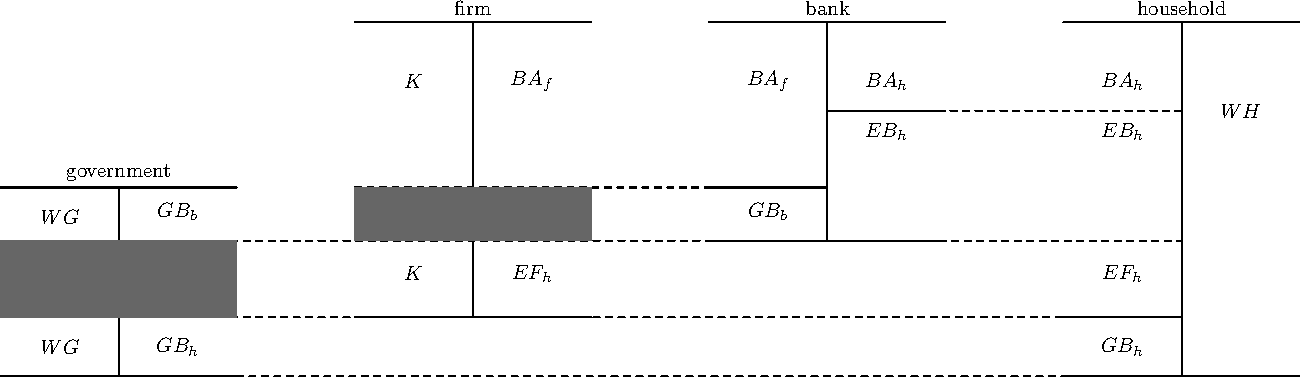
\includegraphics[scale=0.8]{balances-4.pdf}
	\caption{visual representation of the stock matrix}
	\label{fig:vstock4}
\end{figure}
\fi

\begin{figure}[ht]
\hskip-3cm
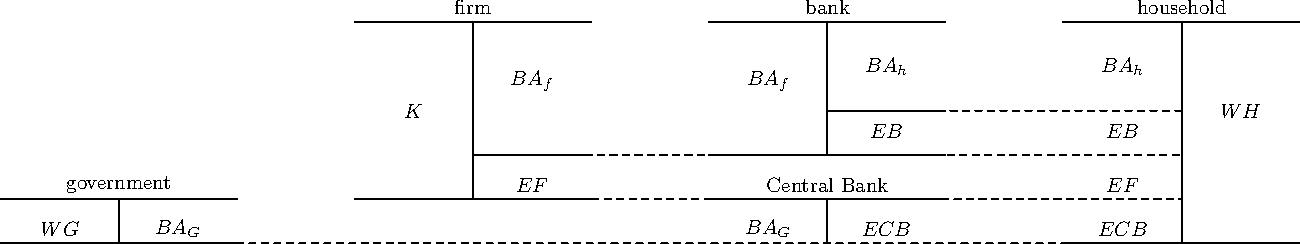
\includegraphics[scale=0.8]{balances-5.pdf}
	\caption{visual representation of the stock matrix}
	\label{fig:vstock5}
\end{figure}



\clearpage
The aggregate stock matrix is obtained by summing over individual values and is reported in table \ref{table:simplified}.

%\vskip5mm
\begin{table}[htp]
\begin{center}
\begin{tabular}{l c c c c c}
	\hline
&	& Household 	& \parbox{1.5cm}{\centerline{Firm}}   & \parbox{1.5cm}{\centerline{Bank}} &$\sum$\\
\hline
\hline
$BA$	&	&$\sum_h BA$	&$\sum_f BA$	&$-\sum_b (\sum_h BA+\sum_f BA)$	&0\\
$E_f$	&	&$\sum_h E_f$	&-$\sum_f E_f$	&$\sum_b E_f$	&0\\
$E_b$	&	&$\sum_h E_b$	&$\sum_f E_b$	&-$\sum_b E_b$	&0\\
	\hline
counterbalance	&&		&	&	&\\
to financial	&&	$\sum_hW$	&$\sum_fK$	&0	&0\\
assets	&&		&	&	&\\
	\hline
	\hline
&$\sum$	&	0	&0	&0	&0\\
\end{tabular}
\end{center}
\caption{A simplified bottom-up stock matrix with a banking sector}
\label{table:simplified}
\end{table}



In each balance sheet, one variable is determined as the complement to the others:

\[
W_h=BA_h+E_b+E_f
\]
\[
E_f=K_f-BA_f+E_b
\]
\[
E_b=\sum BA+E_f
\]

Economic models usually account for the ``normal'' case in which the three variables reported above have positive values. However, it is worth considering ``pathological'' cases in which these variables get negative. This section shed light on how these cases should be treated.  

\newpage 


\end{document}
